%
% teil2.tex -- Beispiel-File für teil2 
%
% (c) 2020 Prof Dr Andreas Müller, Hochschule Rapperswil
%
\section{MiniMax-Polynom 
\label{transfer:section:teil3}}
%\kopfrechts{MiniMax-Polynom}

\subsection{Idee
\label{transfer:subsection:idee}}
Finde das Polynom eines bestimmten Grades, welches eine Funktion
in einem Intervall am besten approximiert. Damit kann der Fehler
bei einem gewissen Rechenaufwand noch einmal verringert werden.

\subsection{Definition
\label{transfer:subsection:definition}}
Das Polynom $P(x)$ welches 
\[
\max _{a \leq x \leq b}|f(x)-P(x)| , a \in \mathbb{R}, b \in \mathbb{R}
\]
minimiert, heisst MiniMax-Polynom von $f$ im Intervall $[a,b]$.
\index{MiniMax-Polynom}%
\kopfrechts{MiniMax-Polynom}

\subsection{Beispiel
\label{transfer:subsection:beispiel}}
Um ein MiniMax-Polynom zu berechnen, kann der Remez-Algorithmus
\index{Remez-Algorithmus}
verwendet werden. Hier wird nicht weiter auf die Berechnung
eingegangen, sondern auf den Wikipedia-Artikel \cite{transfer:remez}
verwiesen.
Für den Tangens hyperbolicus ergibt sich dann für den
Grad 3 im Intervall $[0,3.75]$ das Polynom $P(x)=0.0079+1.0922
x-0.3993 x^{2}+0.0479 x^{3}$.


\begin{figure}
	\centering
	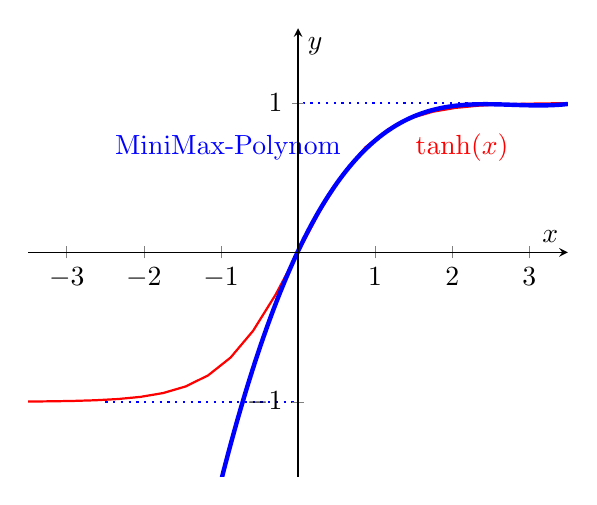
\begin{tikzpicture}
		\begin{axis}[
			xmin=-3.5, xmax=3.5,
			ymin=-1.5, ymax=1.5,
			axis lines=center,
			axis on top=true,
			domain=-3.5:3.5,
			ylabel=$y$,
			xlabel=$x$,
			]
			
			\addplot [mark=none,draw=red,thick] {tanh(\x)};
			\node [right, red] at (axis cs: 1.4,0.7) {$\tanh(x)$};
			\addplot [mark=none,draw=blue,ultra thick, samples=100, smooth] expression{0.0079+1.0922*x-0.3993*x^2+0.0479*x^3};
			\node [right, blue] at (axis cs: -2.5,0.7) {MiniMax-Polynom};
			
			%% Add the asymptotes
			\draw [blue, dotted, thick] (axis cs:-2.5,-1)-- (axis cs:0,-1);
			\draw [blue, dotted, thick] (axis cs:+2.5,+1)-- (axis cs:0,+1);
		\end{axis}
	\end{tikzpicture}
	\caption{MiniMax-Polynom
		\label{motivation:figure:Minimax3}}
\end{figure}

\subsection{Vor- und Nachteile}
Das Minmax-Polynom liefert genau im benötigten Bereich eine gute
Approximation der Funktion.
Wie beim Taylor-Polynom wächst der Fehler aber für $x\to\pm\infty$
polynomiell mit dem Grad des Polynoms an.
Die Minimax-Konstruktion gibt im Vergleich zur Taylor-Approximation
lediglich mehr Kontrolle darüber, in welchem Bereich das
Approximationspolynom gute Resultate liefert.

